\documentclass[../main.tex]{subfiles}
\begin{document}
\subsection{Porte a input singolo}
\begin{figure}[h]
    \centering
    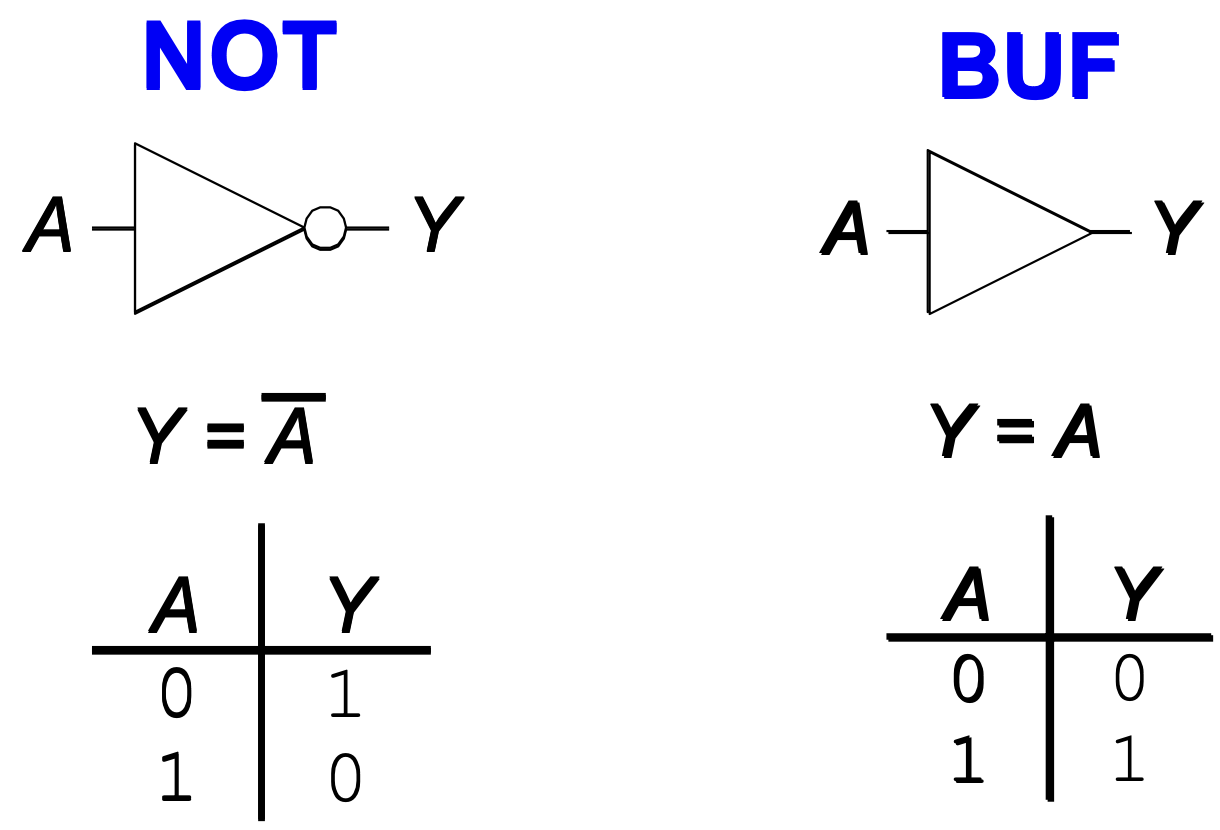
\includegraphics[width=0.4\textwidth]{images/singleInput.png}
    \caption{Porte logiche con un solo input}
\end{figure}
La porta \textbf{NOT} restituisce come output il valore negato rispetto all'input, la porta \textbf{BUF} invece
restituisce la copia del valore di input.

\subsection{Porte a doppio input}
\begin{figure}[h]
    \centering
    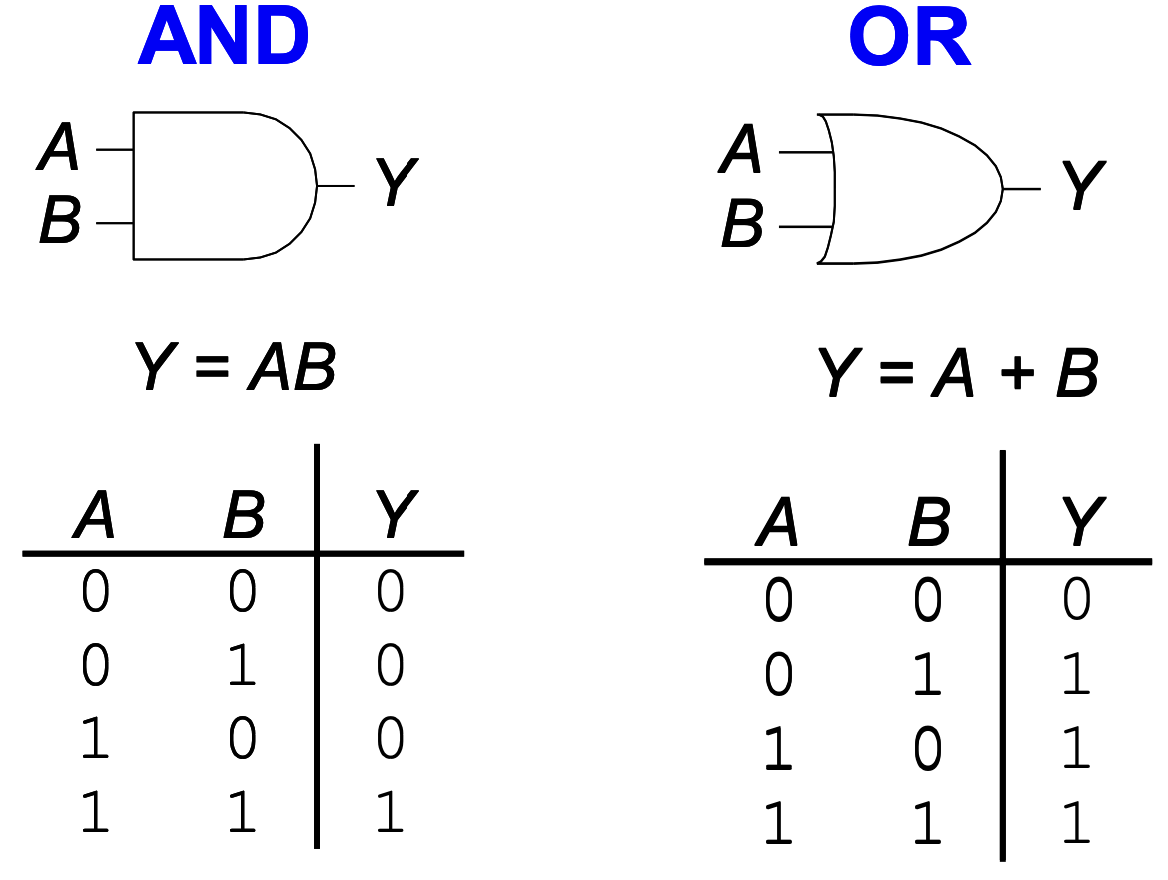
\includegraphics[width=0.4\textwidth]{images/doubleInput.png}
    \caption{Porte logiche con due input}
\end{figure}
La porta logica \textbf{AND} restituisce 1 solo se il valore di entrambi gli input è 1, la porta \textbf{OR} invece
restituisce 1 se almeno uno dei valori di input è 1.

\begin{figure}[h]
    \centering
    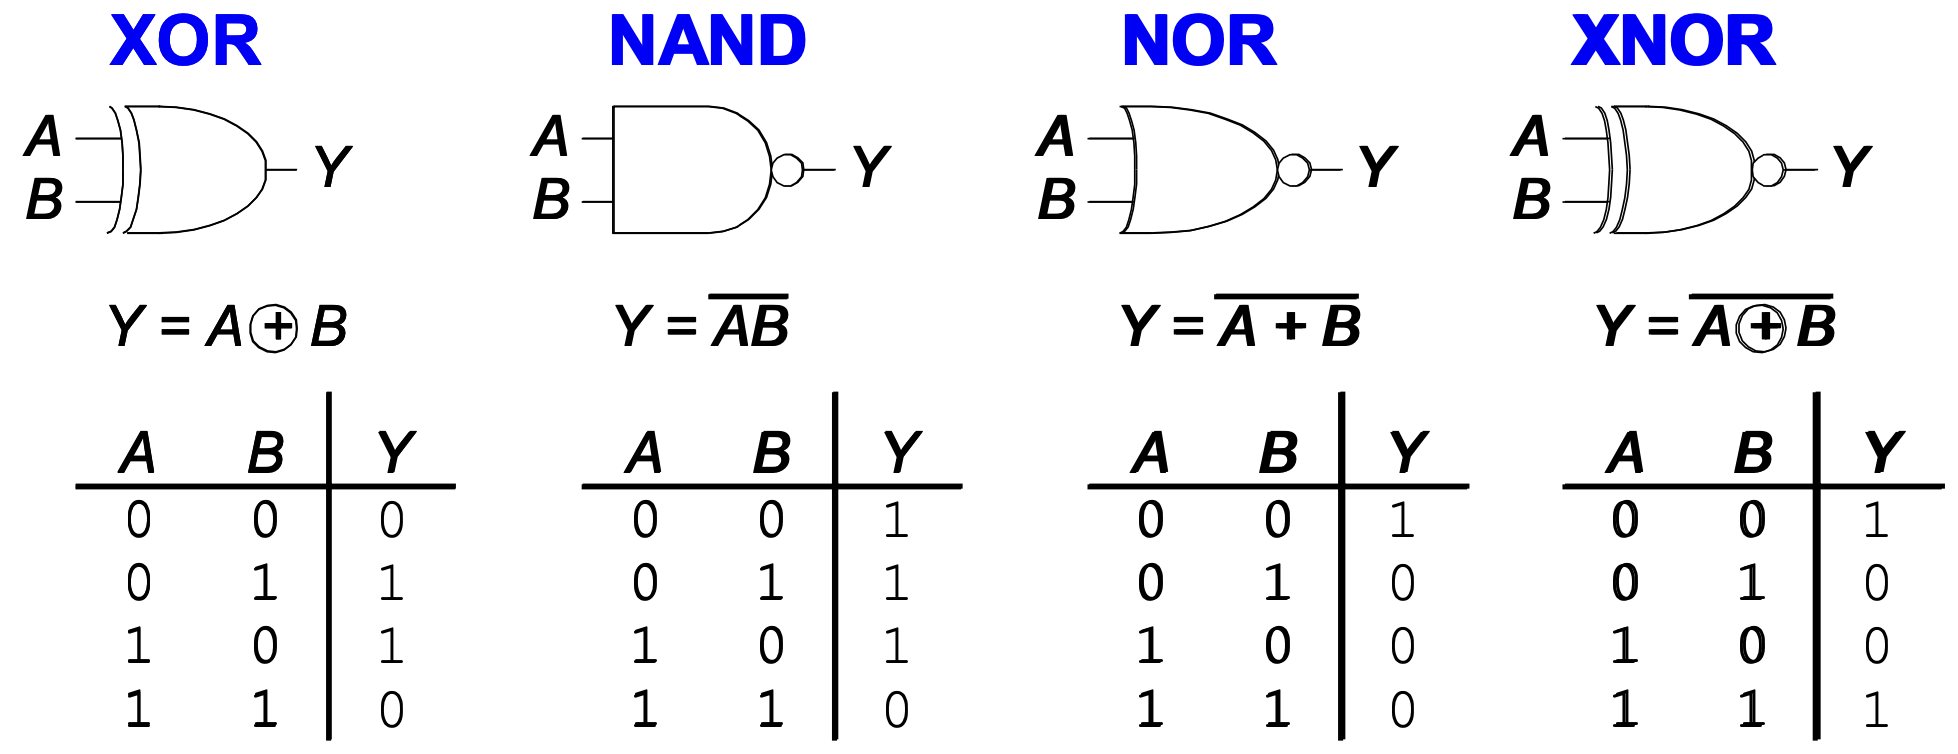
\includegraphics[width=0.4\textwidth]{images/logicGates.png}
    \caption{Altre porte logiche a due input}
\end{figure}
\begin{itemize}
    \item \textbf{XOR}, (\textbf{OR} esclusivo), restituisce 1 solo quando un solo valore di input è 1
    \item \textbf{NAND}, restituisce l'output contrario di una porta \textbf{AND}
    \item \textbf{NOR}, restituisce l'output contrario di una porta \textbf{OR}
    \item \textbf{XNOR}, restituisce l'output contrario di una porta \textbf{XOR}
\end{itemize}

\end{document}